\clearpage

\lehead[]{\normalfont\sffamily\hspace*{-2.00cm}\textcolor{white}{\colorbox{lightblue}{\parbox[c][0.70cm][b]{1.60cm}{
\makebox[1.60cm][r]{\thechapter}\\ \makebox[1.60cm][r]{ÜBUNG}}}}\hspace{0.17cm}\textcolor{lightblue}{\chaptertitle}}
\rohead[]{\textcolor{lightblue}{\chaptertitle}\normalfont\sffamily\hspace*{0.17cm}\textcolor{white}{\colorbox{lightblue}{\parbox[c][0.70cm][b]{1.60cm}{\thechapter\\
ÜBUNG}}}\hspace{-2.00cm}}
%\chead[]{}
\rehead[]{\textcolor{lightblue}{AvHG, Inf, My}}
\lohead[]{\textcolor{lightblue}{AvHG, Inf, My}}

\section{Einfache Dialogelemente -- Übungen}

\subsection{Aufgabe 1: Layout-Manager austesten \tagZusatz}
\noindent \emph{Neues Sprachmittel: Erste Swing-Oberfläche mit dem WindowBuilder erstellen, Layout-Manager vergleichen.}

Teste die beiden wichtigsten Layout-Manager und das NULL-Layout aus, indem du
jeweils eine Anwendung erzeugst, die fünf verschiedene Buttons (mit den
Aufschriften \myUserInput{A}, \myUserInput{B}, \myUserInput{C},
\myUserInput{D} und \myUserInput{E}) mit dem jeweiligen Layout-Manager
anordnet. Beim Klick auf die Buttons soll in dieser einfachen Vorübung noch
nichts geschehen.

\begin{compactenum}[a)]
\item \myClass{FlowLayout}
\item \myClass{GridLayout} mit zwei Zeilen und drei Spalten
\item NULL-Layout
\end{compactenum}


\subsection{Aufgabe 2: Knopfdrücke zählen \tagPflicht}
\noindent \emph{Neues Sprachmittel: Ereignisbehandlung beim \texttt{JButton} (\texttt{ActionListener}) und Textausgabe mit \linebreak \texttt{JLabel.setText()}.}

Programmiere ein \myClass{JFrame} mit einem \myClass{JButton} und einem
\myClass{JLabel}. Gib im Label einen Text aus, der angibt, wie oft der Button
gedrückt wurde. Bei jedem Drücken des Buttons wird der Text angepasst. Verwende
dazu einen Layout-Manager. Ich empfehle das \myClass{FlowLayout}. Du darfst dich
aber auch für einen anderen Layout-Manager entscheiden (nicht NULL-Layout).

\vspace{3mm}

\begin{minipage}{0.75\textwidth}
\subsection{Aufgabe 3: Fahne im Wind \tagZusatz \tagLK}
\noindent \emph{Schwerpunkt: Eigene Zeichenfläche (\texttt{JPanel}) in ein Swing-Fenster integrieren.}

\vspace{4mm}

Zeichne eine Fahne, die je nach Windrichtung nach rechts oder nach links
ausgerichtet ist. Die Windrichtung wird mit einer \myClass{JCheckBox}
ausgewählt. Wenn der Benutzer die Checkbox anklickt, dreht sich die Fahne sofort
in die neue Richtung. Damit die Fahne neu gezeichnet wird, muss im Frame bzw.\
auf der Zeichenfläche die Methode \lstinline|repaint()| aufgerufen werden.
\end{minipage}
\hfill
\begin{minipage}{0.25\textwidth}
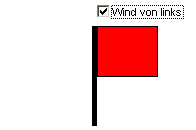
\includegraphics[width=1.0\textwidth]{./inf/SEKII/26_Java_GUI-Komponenten/FahneImWind.png}
\end{minipage}


\subsection{Aufgabe 4: Anrede \tagPflicht}
\noindent \emph{Neues Sprachmittel: Textfelder auslesen (\texttt{JTextField.getText()}) und Auswahlkästchen abfragen \linebreak (\texttt{JCheckBox.isSelected()}).}

Programmiere ein \myClass{JFrame}, das folgendes Aussehen hat:

\begin{center}
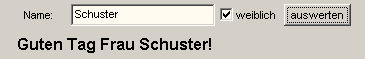
\includegraphics[width=0.6\textwidth]{./inf/SEKII/26_Java_GUI-Komponenten/Anrede.png}
\end{center}

Der Benutzer kann im Textfeld einen Namen eingeben. Wenn man auf den Button
drückt, wird der Benutzer höflich begrüßt. Dabei wird die Checkbox ausgewertet,
um zu ermitteln, ob der Benutzer mit \glqq Frau\grqq\ oder mit \glqq Herr\grqq\
angeredet werden soll. Wenn der Benutzer zum Beispiel den Namen \glqq Meyer\grqq\
eingegeben hat und die Checkbox nicht selektiert ist, wird ausgegeben:
\glqq Guten Tag, Herr Meyer!\grqq


\subsection{Aufgabe 5: RGB-Farben mischen \tagZusatz \tagLK}
\noindent \emph{Schwerpunkt: Zusammenspiel mehrerer GUI-Elemente mit dynamischer Farbberechnung (\texttt{new Color(...)}).}

Programmiere ein \myClass{JFrame}, in dem man die RGB-Werte als Zahlen eingeben
kann. Wenn man auf einen Button drückt, wird mit den eingegebenen RGB-Werten ein
Objekt der Klasse \myClass{Color} erzeugt. Im Konstruktor der Klasse
\myClass{Color} werden als Parameter die drei Farbwerte übergeben. Anschließend
wird die Hintergrundfarbe des \myClass{JFrame}-Fensters (über
\lstinline|getContentPane().setBackground(...)|) auf den gemischten Farbwert
gesetzt (da \myClass{JLabel}-Komponenten standardmäßig durchsichtig sind,
übernehmen sie diese Hintergrundfarbe automatisch).

\begin{minipage}{0.5\textwidth}
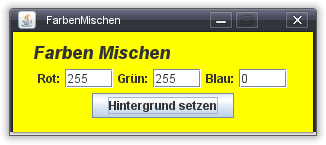
\includegraphics[width=1.0\textwidth]{./inf/SEKII/26_Java_GUI-Komponenten/FarbenMischen.png}
\end{minipage}
\hfill
\begin{minipage}{0.4\textwidth}
\subsubsection{Konvertierung von \myClass{String} nach \myClass{int}}

Beispiel:

\begin{lstlisting}
String text = "77";
int zahl = Integer.parseInt(text);
\end{lstlisting}
\end{minipage}


\section{Anwendungsprojekt: Datenverarbeitung über eine KI-API \tagPflicht}

Moderne Software erledigt komplexe Aufgaben -- wie etwa Spracherkennung,
Übersetzungen oder das Beantworten von Fragen -- selten komplett selbst.
Stattdessen nutzt das eigene Programm über das Netzwerk einen spezialisierten
Dienst. Die dafür bereitgestellte Programmierschnittstelle nennt man
\textbf{API} (\emph{Application Programming Interface}).

\subsection{Wie arbeitet unser Programm mit einer KI-API zusammen?}

Am Beispiel eines eigenen kleinen KI-Assistenten lassen sich gleich zwei
wichtige Sichtweisen der Informationsverarbeitung beobachten:

\begin{compactenum}[1.]
  \item \textbf{Mensch-Maschine-Interaktion (Frontend / GUI):}\\
  Du gibst deine Frage über ein Swing-Eingabefeld (\myClass{JTextField}) ein,
  klickst auf einen \myClass{JButton} und liest die Antwort in einem
  mehrzeiligen Textfeld (\myClass{JTextArea}).
  \item \textbf{Maschine-Maschine-Interaktion (Backend / API):}\\
  Dein Java-Programm verpackt deine Eingabe in ein standardisiertes Datenformat
  (hier: \emph{JSON}) und sendet sie über das Internet an einen KI-Server.
  Dieser berechnet die Antwort und schickt sie an dein Programm zurück.
\end{compactenum}

\medskip
\begin{center}
\fbox{\parbox{0.94\textwidth}{\centering\small
\textbf{Benutzer} $\xrightarrow{\text{Eingabe (GUI)}}$
\textbf{Dein Java-Programm} $\xrightarrow{\text{HTTP / JSON (API)}}$
\textbf{KI-Server} $\xrightarrow{\text{Antwort}}$
\textbf{Dein Programm} $\xrightarrow{\text{Ausgabe (GUI)}}$ \textbf{Benutzer}
}}
\end{center}

\begin{tcolorbox}[colback=blue!5,colframe=lightblue,boxrule=0.8pt,arc=3pt,title={\textbf{Wichtig: Warum hat die KI kein Gedächtnis?}}]
\small
Jeder Aufruf von \lstinline|KIAnfrage.sendePrompt(...)| ist eine eigenständige,
\textbf{zustandslose} (\emph{stateless}) Anfrage. Der KI-Server speichert
deine vorherigen Nachrichten nicht ab. Wenn du nach einer Antwort nur
\glqq Ja, gerne\grqq\ schreibst, weiß die KI nicht mehr, worauf sich das
bezieht. Echte Chat-Programme speichern deshalb den gesamten bisherigen
Verlauf im Client und senden ihn bei jeder neuen Frage komplett wieder mit.
\end{tcolorbox}


\subsection{Die Hilfsklasse \texttt{KIAnfrage} verwenden}

Damit du dich nicht um die technischen Details der Netzwerkverbindung kümmern
musst, stellt dir das Package \texttt{hilfe} die Klasse \myClass{KIAnfrage}
als \emph{Black Box} zur Verfügung. Sie besitzt unter anderem folgende
statische Methoden:

\begin{compactitem}
  \item \lstinline|public static String sendePrompt(String prompt)|\\
  Sendet eine Frage oder Arbeitsanweisung (\lstinline|prompt|) an die KI und
  liefert deren Antwort als \myClass{String} zurück.
  \item \lstinline|public static String sendePrompt(String systemRolle, String prompt)|\\
  Ermöglicht zusätzlich eine Rollenvorgabe (\lstinline|systemRolle|), z.\,B.\
  \glqq Du bist ein freundlicher Informatik-Tutor und antwortest in maximal drei
  Sätzen.\grqq
\end{compactitem}

\medskip
\noindent \textbf{Beispielaufruf im Programm:}
\begin{lstlisting}
import hilfe.*;
...
String antwort = KIAnfrage.sendePrompt("Erkläre den Begriff API in einem Satz.");
textAreaAusgabe.setText(antwort);
\end{lstlisting}

\subsection{Übung: Eigener KI-Assistent mit Swing \tagPflicht}
\noindent \emph{Schwerpunkt: Kombination von Swing-Komponenten (\texttt{JTextField}, \texttt{JButton}, \texttt{JTextArea}) mit einer externen KI-API; Reflexion von Eingabe, Verarbeitung und Ausgabe.}

\begin{compactenum}[a)]
\item Erstelle mit dem WindowBuilder eine grafische Oberfläche für einen
eigenen KI-Assistenten. Sie soll ein Eingabefeld (\myClass{JTextField}) für
deine Frage, einen Button \myUserInput{Frage senden} sowie ein mehrzeiliges
Ausgabefeld (\myClass{JTextArea} innerhalb einer \myClass{JScrollPane}, mit
aktiviertem Zeilenumbruch \lstinline|setLineWrap(true)|) enthalten.

\item Programmiere den \myClass{ActionListener} des Buttons so, dass der
eingegebene Text ausgelesen, über \linebreak \lstinline|KIAnfrage.sendePrompt(...)| an die
KI geschickt und die zurückgelieferte Antwort in der \myClass{JTextArea}
angezeigt wird.

\noindent \textbf{Hinweis (nicht-blockierender Aufruf):} Damit das Fenster
während der Netzwerkanfrage nicht kurz einfriert, bietet \myClass{KIAnfrage}
auch eine asynchrone Variante mit Lambda-Rückruf:
\begin{lstlisting}
taAusgabe.setText("Bitte warten...");
KIAnfrage.sendePromptAsync("Erkläre API.", antwort -> taAusgabe.setText(antwort));
\end{lstlisting}


\item \emph{(Spezialisierung per System-Prompt)} Baue dein Programm zu einem
spezialisierten Helfer um -- z.\,B.\ zu einem \emph{Vokabel-Trainer}, einem
\emph{Code-Erklärer} oder einem \emph{Quiz-Master} --, indem du die zweite
Methode \lstinline|KIAnfrage.sendePrompt(systemRolle, prompt)| nutzt und eine
passende Rollenbeschreibung fest vorgibst.

\item \emph{(Reflexion -- Informatik, Mensch und Gesellschaft)} Diskutiert an
eurem fertigen Programm folgende drei Fragen:
\begin{compactenum}[1.]
  \item Welche Daten verlassen euren Computer bei jeder Anfrage, und was
  bedeutet das für den \textbf{Datenschutz} (z.\,B.\ bei personenbezogenen
  Eingaben)?
  \item Warum liefert die KI auf dieselbe Frage manchmal leicht
  unterschiedliche Antworten (\emph{Probabilität} statt fester
  Programmregeln), und warum darf man ihre Aussagen nicht ungeprüft
  übernehmen?
  \item Welche Vorteile bietet die Trennung zwischen eurer lokalen
  Benutzeroberfläche (Frontend) und dem KI-Dienst über eine API (Backend)?
\end{compactenum}
\end{compactenum}


